\section{Introduction}

The most common definitions of fairness in machine learning are statistical in nature. 
They proceed by fixing a small number of ``protected subgroups'' (such as racial or gender groups), and then ask that some statistic of interest be approximately equalized across groups. Standard choices for these statistics include positive classification rates \citep{CV10}, false positive or false negative rates \citep{HPS16,KMR16,Chou16} and positive predictive value \citep{Chou16,KMR16} --- see \cite{Berksurvey} for more examples. These definitions are pervasive in large part because they are easy to check, although there are interesting computational challenges in learning subject to these constraints in the worst case --- see e.g. \cite{hardnesspaper}.

%and so many previous approaches have necessarily taken heuristic approaches to learning the optimal fair classifier. These approaches include relaxation of the fairness constraints by enforcing a weaker constraint (decorrelating the protected feature and classifier for example), the related approach of adding a \textit{fairness regularizer} to the optimization objective, and pre-processing of the data or post-processing of a black-box classifier \cite{} \ar{Blue box?}. Enforcing heuristic constraints both forces the practitioner to substantially change the training algorithms used -- a potential barrier to adoption in practical machine learning pipelines -- and fails to optimize for the desired fairness criterion except under stylized assumptions about the hypothesis class, data, or training algorithm used. Post-processing enjoys ease of integration with a black-box learner, but has limited theoretical justification \cite{hardnesspaper}. The recent work of \cite{MSR} provides a definitive improvement over these prior approaches, giving a practical algorithm for learning the optimal fair classifier under the common statistical fairness notions, while reducing the problem to an iterative sequence of black-box calls to a learner for the underlying classification problem. Under the assumption that the black-box learner succeeds, the algorithm provably quickly converges to the optimal fair classifier. Due to both the prevalence of statistical fairness notions in the literature, and the clear advantages of this method over prior approaches to learning subject to statistical fairness constraints, \cite{MSR} is the state-of-the-art algorithm for learning optimally accurate fair classifiers (with access to demographic features).



 Unfortunately, these statistical definitions are not very meaningful to individuals: because they are constraints only over \emph{averages} taken over large populations, they promise essentially nothing about how an individual person will be treated. \citet{awareness} enumerate a ``catalogue of evils'' which show how definitions of this sort can fail to provide meaningful guarantees. \citet{KNRW18} identify a particularly troubling failure of standard statistical definitions of fairness, which can arise naturally without malicious intent, called ``fairness gerrymandering''. They illustrate the idea with the following toy example shown in Figure \ref{fig:example}, described as follows.
 \begin{figure}
\centering
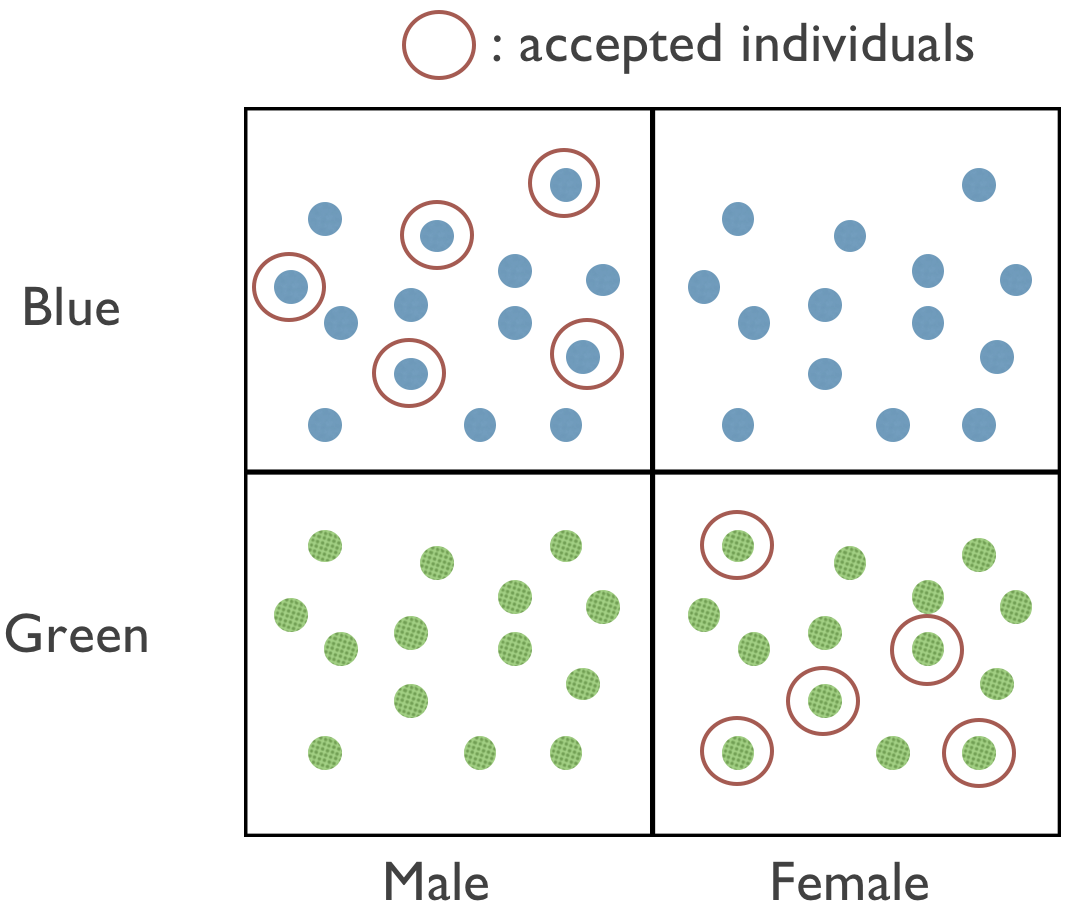
\includegraphics[scale=0.3]{figures/subgroups.png}
\caption{Fairness Gerrymandering: A Toy Example \citep{KNRW18}}
\label{fig:example}
\end{figure}

Suppose individuals each have two sensitive attributes: race (say blue and green) and gender (say male and female). Suppose that these two attributes are distributed independently and uniformly at random, and are uncorrelated with a binary label that is also distributed uniformly at random. If we view gender and race as defining classes of people that we wish to protect, we could take a standard statistical fairness definition from the literature --- say the equal odds condition of \cite{HPS16}, which asks to equalize false positive rates across protected groups, and instantiate it with the four protected groups: ``Men'', ``Women'', ``blue people'', and ``green people''. The following classifier satisfies this condition, although only by ``cheating'' and packing its unfairness into structured subgroups of the protected populations: it labels a person as positive only if they are a blue man or a green woman. This equalizes false positive rates across the four specified groups, but of course not over the finer-grained subgroups defined by the intersections of the two protected attributes.


\citet{KNRW18} also proposed an approach to the problem of fairness
gerrymandering: rather than asking for statistical definitions of
fairness that hold over a small number of coarsely defined groups, ask
for them to hold over a combinatorially or infinitely large collection
of subgroups defined by a set of functions $\cF$ of the protected
attributes (\citet{multical} independently made a similar
proposal). For example, we could ask to equalize false positive rates
across every subgroup that can be defined as the intersection or
conjunction of $d$ protected attributes, for which there are $2^d$
such groups. \cite{KNRW18} showed that as long as the class of
functions defining these subgroups has bounded VC dimension, the
statistical learning problem of finding the best (distribution over)
classifiers in $\cH$ subject to the constraint of equalizing the
positive classification rate, the false positive rate, or the false
negative rate over every subgroup defined over $\cF$ is solvable
whenever the dataset size is sufficiently large relative to the VC
dimension of $\cF$ and $\cH$. Taking inspiration from the technique of
\citet{MSR}, they were able to show that even with
combinatorially many subgroup fairness constraints, the computational
problem of learning the optimal fair classifier is once again solvable
efficiently whenever the learner has access to a black-box classifier
(oracle) which can solve the \emph{unconstrained} learning problems
over $\cF$ and $\cH$ respectively. Similarly, given access to an
oracle for $\cF$, they were able to efficiently solve the problem of
\textit{auditing} for rich subgroup fairness: finding the $g \in \cF$
that corresponds to the subgroup for whom the statistical fairness
constraint was most violated.

While the work of \citet{KNRW18} is satisfying from a theocratical point of view, it leaves open a number of pressing empirical questions. For example, their theory is built for an idealized setting with perfect learning oracles --- in practice heuristic oracles may fail. Moreover, perhaps rich subgroup fairness is asking for too much in practice --- maybe enforcing combinatorially many constraints leads to an untenable tradeoff with error.  Finally, perhaps enforcing combinatorially many constraints is not necessary --- perhaps on real data, it is enough to call upon the algorithm of \cite{MSR} for enforcing statistical fairness constraints on the small number of groups defined by the marginal protected attributes, and rich subgroup fairness will follow incidentally. Put another way: Is the so-called \textit{fairness gerrymandering} problem only a theoretical curiosity, or does it arise organically when standard classifiers are optimized subject to marginal statistical fairness constraints?

In this paper, we conduct an extensive set of experiments to answer these questions. We study the algorithm from \cite{KNRW18} --- instantiated with fast heuristic learning oracles --- when used to train a linear classifier subject to approximately equalizing false positive rates across a rich set of subgroups defined by linear threshold functions. On four real datasets, we characterize:

%In this paper we conduct a diverse and detailed study of a statistical fairness notion and linear classifier on four fairness-sensitive datasets, tracing out a fairness-error Pareto curve, and providing a detailed comparison to optimizing for marginal fairness using the algorithm of \cite{MSR}. We call our notion of fairness \emph{rich subgroup fairness} with respect to a class $\cF$, and in this paper always instantiate it with \emph{false positive rates} as the statistic that we equalize across subgroups. We characterize:

\begin{enumerate}
\item The basic convergence properties of the algorithm --- although this algorithm has provable guarantees when instantiated with learning \emph{oracles} for $\cF$ and $\cH$, when these oracles are (necessarily) replaced with heuristics, the guarantees of the algorithm become heuristic as well. We find that the algorithm typically converges (Subsection~\ref{subsec:conv}), and provides a controllable trade-off between fairness and accuracy despite its heuristic guarantees (Subsection~\ref{subsec:Pareto}). We visualize the optimization trajectory of the algorithm (Subsection~\ref{subsec:traj}), and \textit{discrimination heatmaps} showing the evolution of the subgroup discrimination of the algorithm over time (Subsection~\ref{subsec:heatmap}).
    \item The trade-off between subgroup fairness and accuracy. We find that for each dataset, there are appealing compromises between
	error and subgroup fairness. Thus achieving rich subgroup fairness may be possible in practice
	without a severe loss in predictive accuracy (Subsection~\ref{subsec:Pareto}).
\item The subgroup (unfairness) that can result when one applies more standard approaches, that either ignore fairness constraints all together, or equalize false positive rates only across a small number of subgroups defined by individual protected attributes. By \textit{auditing} the models produced by these standard approaches with the rich subgroup auditor of \cite{KNRW18}, we find that often subgroup fairness constraints are violated, even by algorithms which are explicitly equalizing false positive rates across the groups defined on the marginal protected attributes.
%\item Interestingly, in all datasets but one,  minimizing marginal unfairness monotonically minimizes subgroup unfairness as well -- albeit with a worse error-fairness tradeoff than by directly optimizing for rich subgroup fairness via the algorithm of \cite{KNRW18}.
\end{enumerate}

In light of these findings, we submit that rich subgroup fairness constraints are both important, and can be satisfied at reasonable cost: both in terms of computation, and in terms of accuracy. We hope that algorithms like that of \cite{KNRW18} which can be used to satisfy rich subgroup fairness become part of the standard toolkit for fair machine learning. 
%Towards this end, we provide our open-source implementation of the algorithm of \cite{KNRW18} (\textbf{Not provided in submission version to satisfy double blind review}.)

\subsection{Further Related Work}
While \citet{KNRW18} propose and study rich sub-group fairness for false positive and negative constraints, \citet{multical} study the analogous notion for \emph{calibration} constraints, which they call \emph{multi-calibration}. \citet{multiac} extend this style of analysis to \emph{accuracy} constraints (asking that a classifier be equally accurate on a combinatorially large collection of subgroups). \citet{multimet} also extend it to metric fairness constraints, converting the \emph{individual} metric fairness constraint of \citet{awareness} into a statistical constraint that asks that \emph{on average}, individuals in (combinatorially many) subgroups should be treated differently only in proportion to the average difference between individuals in the subgroups, as measured with respect to some similarity metric.


%
%\begin{itemize}
%\item Standard fairness notions in ML/stats are statistical in nature,
%	only provide guarantees at level of course groups
%\item Example: equality of FN across races in lending
%\item Can't expect to make such promises at individual level without
%	perfect predictions
%\item But might hope to avoid ``fairness gerrymandering'': meet
%	coarse group-level constraint by discriminating against
%	fine-grained subgroups
%\item Example: protect race, age, gender, disability separately but
%	find discrimination against disabled Hispanic women over age 55
%\item Relation to intersectionality
%\item Preventing would provide much stronger/satisfying fairness
%	guarantees --- {\em rich subgroup fairness (SSF)}
%\item We recently developed algorithms that provably find
%	error-optimal models satisfying (approximate) SSF
%\item But the trade-off between error and SSF can only be studied
%	empirically, and may vary across datasets
%\item In this paper we demonstrate that SSF is a practical goal
%	via extensive experiments on four different fairness-sensitive
%	datasets
%\item For each dataset we show there are appealing compromises between
%	error and SSF, thus achieving SSF may be possible in practice
%	without much loss in predictive accuracy
%\item We compare our algorithm to more standard approaches, and offer
%	insights into its behavior/dynamics
%\item We believe/hope algo and SSF can become standard tools for fair ML,
%	will provide open-source code
%
%
%
%
%\end{itemize} 
%%% Local Variables:
%%% mode: latex
%%% TeX-master: "main"
%%% End:
